
\section{Demonstration project}
    The aim of the demonstration project is to provide an easy way to explore the IDE without reading long documents. The demonstration project can be opened from the welcome dialog ( Main Menu Help Welcome dialog Open demonstration project. ) Demonstration project should introduce new user into usage of the most common functions of the IDE like assembling the code, running simulator and so on. Demonstration project cannot be modified by the user.
    \begin{figure}[h]
        \centering{}
        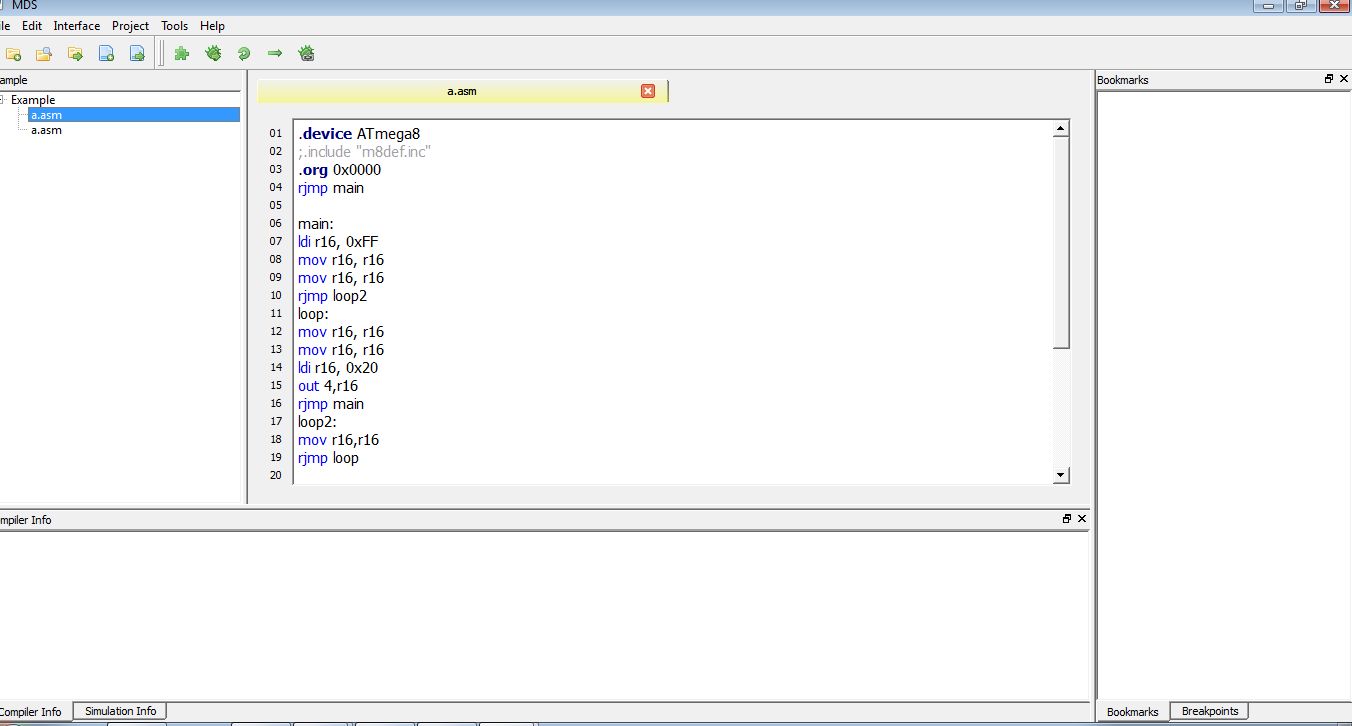
\includegraphics[width=.5\textwidth]{img/Demonstration_project.png}
        \caption{Demonstration project}
    \end{figure}

\section{Your first project}
    There is actually not too much you have to do in order to start you first project. To keep things simple:
    \begin{itemize}
        \item Click on "New project" either on the Welcome screen, or in the main menu (submenu Project).
        \item Choose a name for your project and directory in which you want to store files created in the IDE.
        \item Click on "New file" main menu (submenu File), write your code, click on "Save", choose a name.
        \item Click on "Compile".
        \item Click on "Start simulation", and press "Step" repeatedly to see actual simulation.
        \item Compiled files suitable for loading into FPGA can be found in the directory which you choose to be your project directory.
    \end{itemize}

    \begin{figure}[h]
        \centering{}
        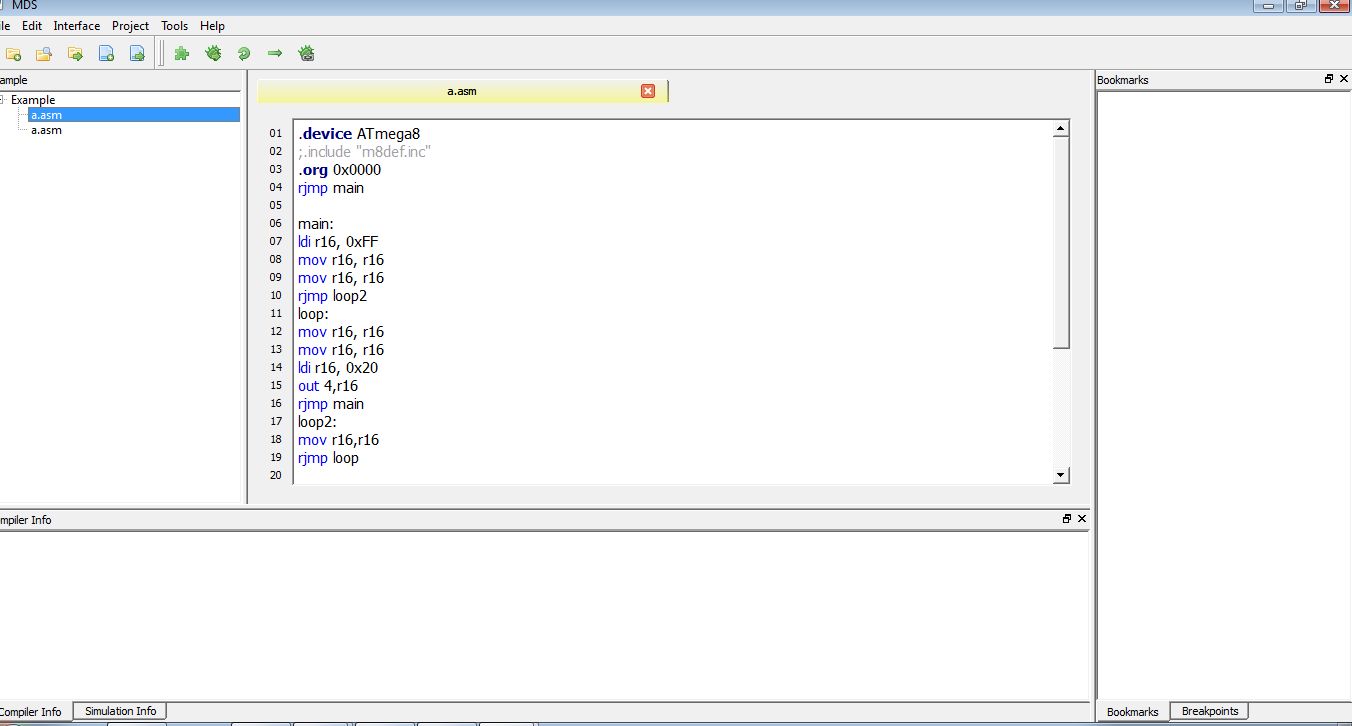
\includegraphics[width=.5\textwidth]{img/Demonstration_project.png}
        \caption{Demonstration project}
    \end{figure}

\section{What is PicoBlaze?}
    PicoBlaze is the designation of a series of three free soft processor cores from Xilinx for use in their FPGA and CPLD products. They are based on a RISC architecture of 8 bits and can reach speeds up to 100 MIPS on the Virtex 4 FPGA"s family. The processors have an 8-bit address and data port for access to a wide range of peripherals. The license of the cores allows their free use, albeit only on Xilinx devices, and they come with development tools. All instructions execute in two clock cycles, making performance of the core instruction set deterministic. Interrupt response is not more than five clock cycles. As a resource optimization, it is possible for two PicoBlaze cores to share the same instruction PROM, taking advantage of the dual-ported implementation of this block on Xilinx FPGAs.

    \paragraph{PicoBlaze features:}
        \begin{itemize}
            \item Harvard architecture processor core customizable to fit user specific requirements.
            \item General-purpose data registers.
            \item Byte-wide Arithmetic Logic Unit (ALU) with CARRY and ZERO indicator flags.
            \item Optional internal scratchpad RAM.
            \item 256 input and output ports for easy expansion and enhancement.
            \item Automatic CALL/RETURN stack.
            \item Predictable performance, always two clock cycles per instruction, up to 200 MHz or 100 MIPS in a Virtex-II Pro FPGA.
            \item Fast interrupt response; worst-case 5 clock cycles.
            \item Optimized for Xilinx FPGAs.
        \end{itemize}
